\begin{figure}[htbp]
\centering
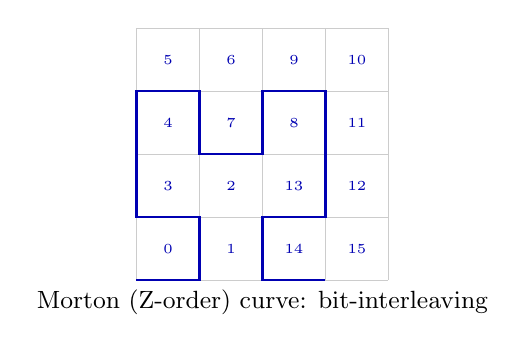
\begin{tikzpicture}[scale=0.8]
  \draw[gray!40,thin] (0,0) grid (4,4);
  \draw[blue!70!black,thick] (0,0)--(1,0)--(1,1)--(0,1)--(0,2)--(0,3)--(1,3)--(1,2)--(2,2)--(2,3)--(3,3)--(3,2)--(3,1)--(2,1)--(2,0)--(3,0);
  \foreach \x/\y/\c in {0/0/0, 1/0/1, 1/1/2, 0/1/3, 0/2/4, 0/3/5, 1/3/6, 1/2/7, 2/2/8, 2/3/9, 3/3/10, 3/2/11, 3/1/12, 2/1/13, 2/0/14, 3/0/15} {
    \node[font=\tiny,blue!70!black] at (\x+0.5,\y+0.5) {\c};
  }
  \node[below,font=\small] at (2,0) {Morton (Z-order) curve: bit-interleaving};
\end{tikzpicture}
\caption{Morton curve: the Z-shaped traversal is obtained by interleaving the binary representations of $x$ and $y$.}
\label{fig:morton_curve}
\end{figure}
